\documentclass{article}           %% ceci est un commentaire (apres le caractere %)
\usepackage[utf8]{inputenc}   
%on me dit : usepackage avec l'option [latin1] mais ça foire... donc je prends utf8, du moment que c beau
\usepackage[T1]{fontenc}          %% permet d'utiliser les caractères accentués
\usepackage[french]{babel}
\usepackage[pdftex]{graphicx}
\usepackage{graphics}

\usepackage{graphics}
\usepackage{fancybox}		   %% package utiliser pour avoir un encadré 3D des images
\usepackage{fancyhdr}
\usepackage{makeidx}              %% permet de générer un index automatiquement
\usepackage[style=numeric,backend=bibtex]{biblatex}				%% Utilisé pour la biblio
\usepackage[top=3cm, bottom=4cm, left=2cm, right=2cm,headsep = 0.5cm,headheight = 1cm, footskip = 1cm,marginparsep = 0cm,marginparwidth=0cm]{geometry} %%pour aller vite


\pagestyle{fancy}
\renewcommand\headrulewidth{1pt}
\fancyhead[L]{Document de travail}
\fancyhead[R]{Octobre 2014}
\fancyfoot[L]{}
\fancyfoot[R]{}



\title{Notre beau réseau de concepts}     %% \title est une macro, entre { } figure son premier argument
\author{Proposition de Schrotty accompagné de diagrammes}        %% idem
\date{Octobre 2014}

\begin{document}
\maketitle

\section{Ce qu'on garde de Copycat/BAsCET et ce qu'on ne garde pas}

On garde :
\begin{itemize}
 \item Le réseau de concepts (RC)
 \item Les activations des noeuds, leur propagation selon leur similarité
 \item Le "workspace" dans lequel des instances des noeuds du réseau de concepts sont créées et reliées entre elles
\end{itemize}

On ne garde pas :
\begin{itemize}
 \item Pas trop d'aléatoire : le programme ne doit pas faire preuve d'initiative, mais de synthèse
 \item Pas de salle d'attente stochastique pour les codelets (pas de sélection aléatoire de ceux-ci)
 \item Pas de codelets ?
\end{itemize}


\section{Développement sur un exemple}
\subsection{Du texte}

From <http://www.bbc.com/sport/0/football/28947896>\\

Wayne Rooney celebrated his appointment as England captain with the winner against Norway on a night when fans turned their back on the team following their dismal World Cup exit.\\

Only 40,181 turned out at Wembley for England's first game since they were eliminated after two group-stage defeats by Italy and Uruguay in Brazil.

Rooney's penalty at least enabled manager Roy Hodgson to enjoy the taste of victory after a winless summer in South America - but the lowest turn-out for an England international at the new Wembley underlined the extent to which England have lost the public's imagination.

Norway are hardly the most glamorous of opponents, but on a balmy night such a meagre attendance is a reflection on the apathy that currently surrounds the England team after the World Cup.

This game was designed as preparation for Monday's testing Euro 2016 qualifier against Switzerland in Basel and it was an uninspiring affair played out in front of vast swathes of empty seats, with Wembley's top tier deserted and the one below hardly populated.

\subsection{Réseau de concepts associé}

Le réseau de concept peut être mis sur pied automatiquement (et complété plus tard).
Les proximités conceptuelles peuvent être calculées automatiquement à la louche.

Sur mon exemple je reprends :
\begin{itemize}
 \item La proximité conceptuelle (de 0 à 100, à 100 c'est des synonymes)
 \item Le fait que les noeuds du RC peuvent aussi être sur des liens du RC (l'activation de noeuds présents sur des liens augmente la proximité conceptuelle de ces liens)
 \item Le taux d'activation (de 0 à 100, à 100 c'est la fête)
\end{itemize}


\subsection{Exécution du programme}

Pour bien voir, je subdivise arbitrairement ma phrase en trois blocs :
\begin{enumerate}
  \item \verb|Wayne Rooney, celebrated, his appointement, as, England captain, |
  \item \verb|with, the winner, against, Norway |
  \item \verb|on, a night, when, fans, turned their back, on, the team|
\end{enumerate}

 A chaque mot, un nouveau tour de programme qui comprend :
 \begin{itemize}
  \item L'activation du noeud correspondant dans le RC
  \item La propagation de cette activation aux noeuds voisins. Ex. : à la lecture de \textit{Wayne Rooney}, le noeud \textit{football} est aussi activé
  \item La création d'objets dans le workspace pour tous les noeuds d'activation suffisante (noter que pour le moment, je ne considère pas d'instances mutliples)
  \item La modification des proximités entre noeuds du RC en fonction de l'activation des noeuds qui sont sur les liens
 \end{itemize}
 
\begin{figure}[htp]
 \centering
  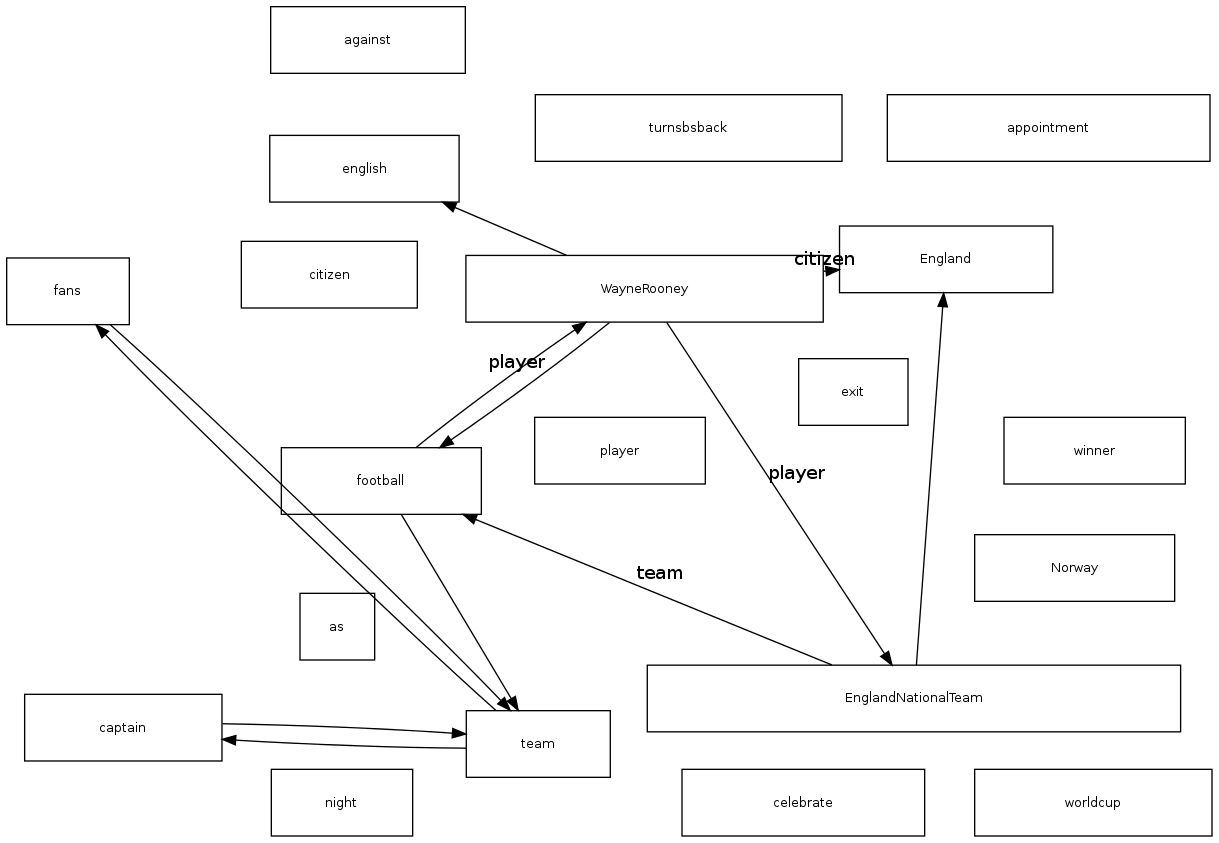
\includegraphics[width=\textwidth]{RCetape0.eps}
 \caption{Réseau de concepts initial}
 \label{fig:RC0}
\end{figure}

 

 
 \subsection{Etape 1}
 Les noeuds sont activés, je propage les activations aux noeuds voisins à la louche, il y a une très bonne formule pour faire tout intervenir en même temps. Pour que ce soit plus lisible je désactive plusieurs noeuds d'un coup.

 Miracle, à ce moment sont activés en priorité les noeuds : Wayne Rooney, England, Captain, appointment ; ainsi que celebrate et football.
 
 \textit{Appointment} et \textit{celebrate} vont plus rapidement se désactiver, car leur importance (profondeur) est faible.

\begin{figure}[htp]
 \centering
  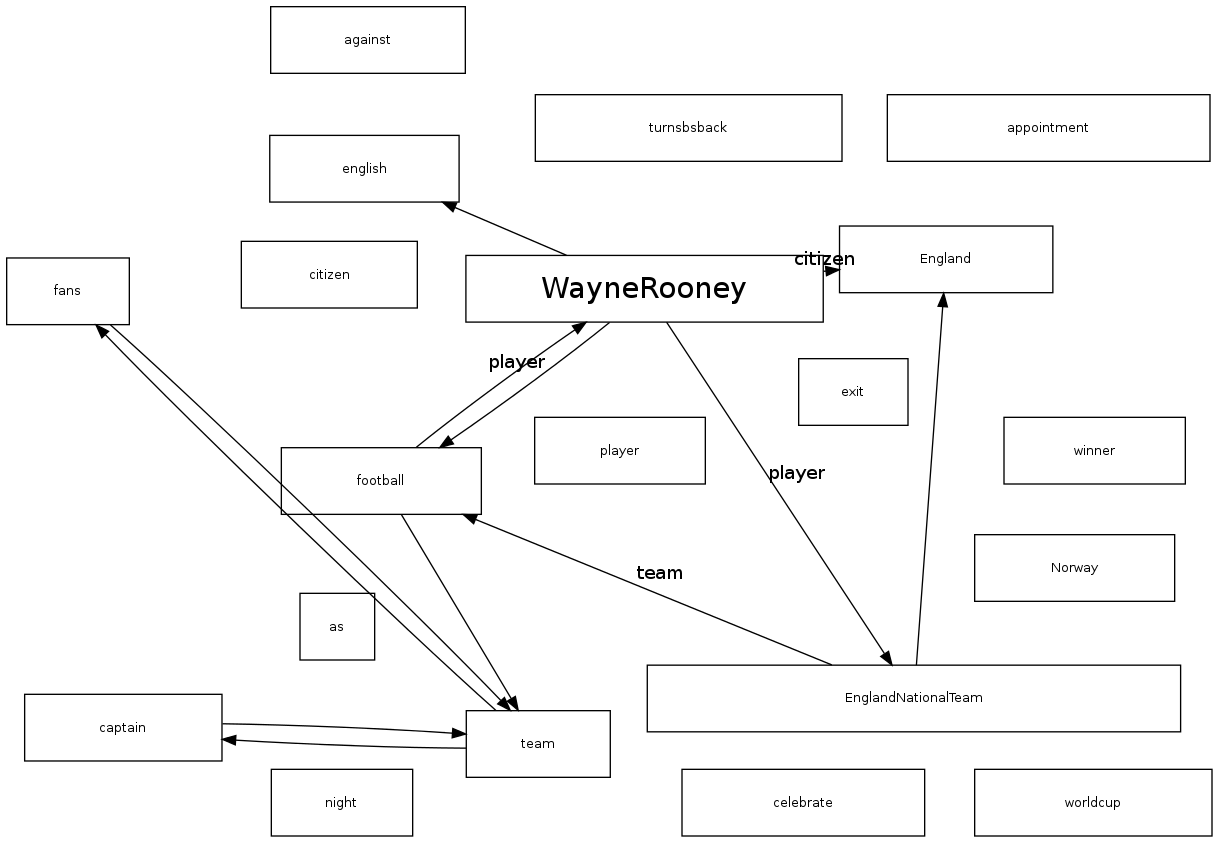
\includegraphics[width=\textwidth]{RCetape1.eps}
 \caption{Réseau de concepts étape 1}
 \label{fig:RC1}
\end{figure}

\begin{figure}[htp]
 \centering
  \includegraphics[width=0.6\textwidth]{workspace1.eps}
 \caption{Workspace étape 1}
 \label{fig:W1}
\end{figure}


 \subsection{Etape 2}

 Je continue avec le deuxième morceau de phrase. Le principe est que les noeuds perdent de l'activation, mais restent au fur et à mesure en sommeil.
 
 \begin{figure}[htp]
 \centering
  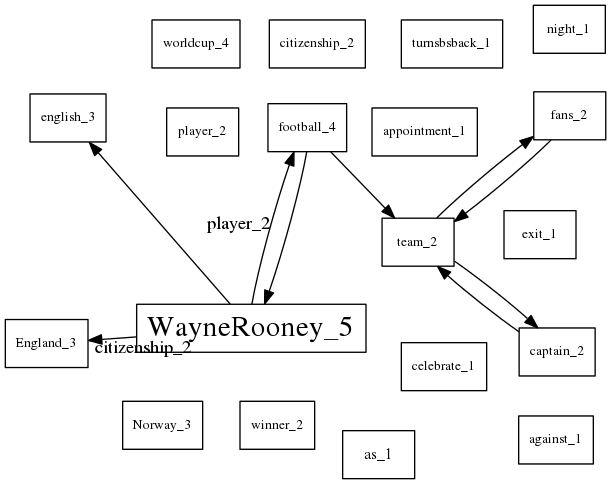
\includegraphics[width=\textwidth]{RCetape2.eps}
 \caption{Réseau de concepts étape 2}
 \label{fig:RC2}
\end{figure}

\begin{figure}[htp]
 \centering
  \includegraphics[width=\textwidth]{workspace2.eps}
 \caption{Workspace étape 2}
 \label{fig:W2}
\end{figure}



 \subsection{Etape 3}

 \begin{figure}[htp]
 \centering
  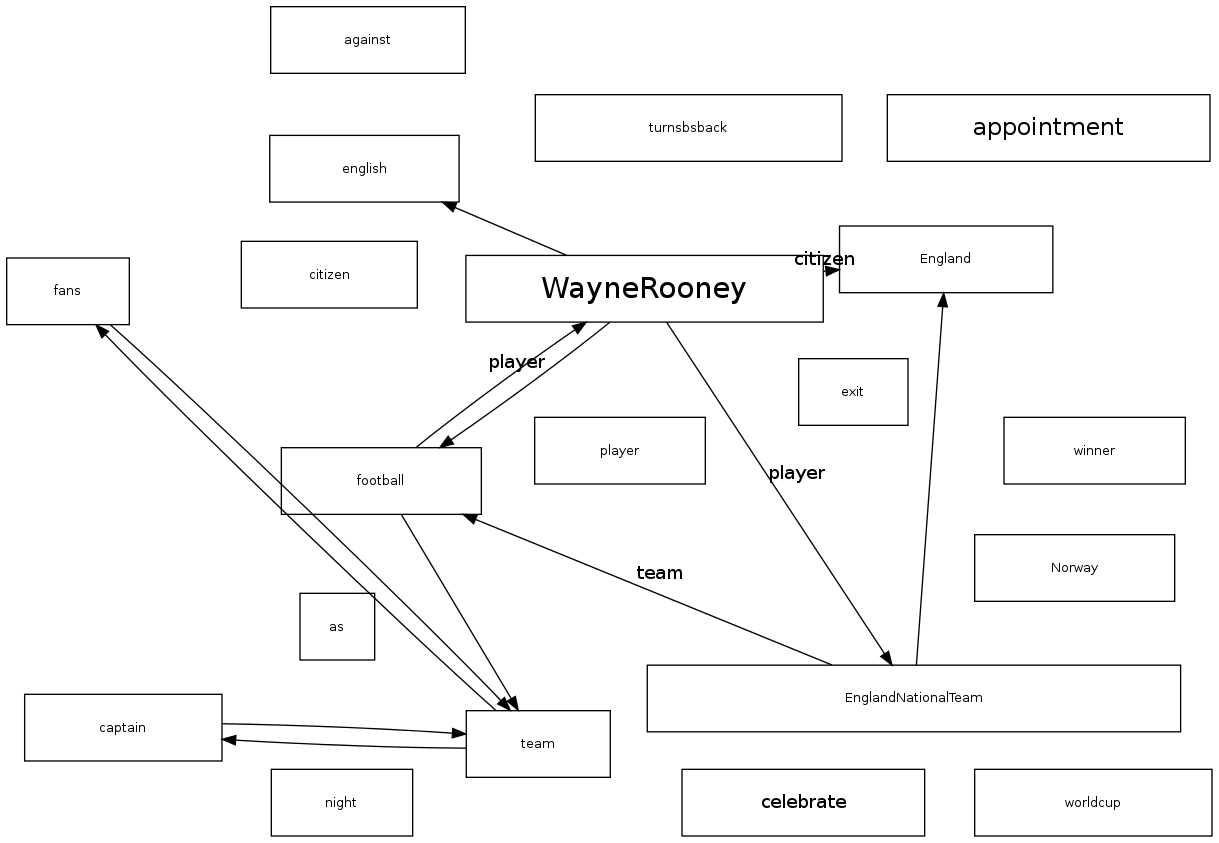
\includegraphics[width=\textwidth]{RCetape3.eps}
 \caption{Réseau de concepts étape 3}
 \label{fig:RC3}
\end{figure}
 
 \begin{figure}[htp]
 \centering
  \includegraphics[width=\textwidth]{workspace3.eps}
 \caption{Workspace étape 3}
 \label{fig:W3}
\end{figure}

 
 Comme ce n'est pas clair du tout, prenons des exemples de noeuds :
 \begin{itemize}
  \item Le noeud \textit{captain} : activé une première fois, il s'est désactivé lentement car c'est un noeud d'assez grande importance. Il a été réactivé par propagation de l'activation du noeud team. A la fin de la lecture, c'est donc un noeud d'assez grande importance
  \item Le noeud \textit{Wayne Rooney} : forte importance conceptuelle et beaucoup de voisins (c'est un paramètre à prendre naturellement en compte, pas sur mon exemple qui est trop petit). Il se désactive peu vite et il est réactivé à chaque fois qu'on parle de WR ou de quelque chose de proche... c'est-à-dire dans tout l'article
  \item Le noeud \textit{England} : d'importance égale à \textit{Norway}, il se désactivera moins vite car l'activation d'autres noeuds se propage vers lui (il est plus question de l'angleterre que de la norvège dans cet article)
 \end{itemize}

La construction réalisée dans le workspace : je vous accorde qu'elle dépend un peu de l'information grammaticale qu'on a pu obtenir. Mais c'est assez souple.

Figure \ref{fig:Wf} : je souligne l'activation des noeuds correspondants.

\begin{figure}[htp]
 \centering
  \includegraphics[width=\textwidth]{workspacef.eps}
 \caption{Workspace final}
 \label{fig:Wf}
\end{figure}



\subsection{Bilan}
\begin{itemize}
 \item Clairement, l'information la plus importante c'est que WR a été nommé capitaine. Mais rien n'empêche une réactivation des autres noeuds lors de la lecture de la suite de l'article ;
 \item Le terme celebrated a été viré !!! Je suis très content de ça car il ne nous sert à rien ;
 \item Vous pouvez dire que j'ai tout bidouillé pour que ça fonctionne, c'est exact ;
 \item Mon exemple est très réduit, mais de nombreux liens existent dans le RC (liens récupérés après une analyse type TF-IDF de proximité conceptuelle), donc avec tous ces liens et toutes ces activations, je pense que le résultat est vraiment pas mal (contrairement au mien où je n'ai même pas fait les calculs correctement) ;
 \item Je pense (c'est personnel :) ) que nous n'avons pas besoin des codelets. En tout cas, on a déjà suffisamment d'embrouilles avec de la propagation d'activations.
\end{itemize}

\subsection{Des détails sur l'implémentation possible}

\paragraph{D'où viennent les noeuds du RC ?}
\begin{itemize}
 \item De FreeBase
 \item De notre TF-IDF pour les concepts importants
 \item Pour tous les mots d'usage courants sur lesquels on tombe, il faut créér des concepts correspondants. Cela peut se faire sur place. Ces mots sont reconnus et la synonymie est reconnue à l'aide de WordNet (utilisable directement avec nltk)
\end{itemize}

\paragraph{D'où viennent les informations de base sur les noeuds du RC ?}
\begin{itemize}
 \item A l'intérieur d'une même phrase, ou d'une même proposition, si deux concepts ont tendance à être tous les deux souvent présents, leur proximité augmente en conséquence. On peut le faire sur une étude statistique
 \item On peut aussi ajouter des infos "à la main" si nécessaire
 \item FreeBase pourvoit aussi en informations sur un certain nombre de nos concepts (comme il y aura beaucoup de noms...)
\end{itemize}

 
\end{document}
